The manuscripts contained within this thesis present the creation and application of infrastructure and
methodology for the analysis of stability in neuroimaging pipelines, and demonstrate their application for both
the study of robustness in an analytical context and the generation of more generalizable brain-phenotype
relationships. These four manuscripts incrementally present the methods developed to perform a large scale
evaluation of numerical stability in neuroimaging, each providing a foundation for the following studies. As a
result, this thesis has led to the creation of both scientific software resources and considerable scientific
advancement in the study of numerical stability in neuroimaging.

In the following sections I will discuss and interpret the findings as a whole and their implications on the field
of structural connectomics. I will then discuss the relevance of extrapolating these conclusions to other domains
of neuroimaging, including the analysis of both functional and structural images. Beyond discussing the
implications of the results presented here, I will propose ways in which perturbation analyses may be further
adopted in neuroimaging, and conclude with lessons learned both from my own pursuit of these projects and
recommendations for the field at large.

\subsection{The Impact of Perturbing Structural Connectome Estimation}

Throughout this thesis I have demonstrated that controlled perturbations serve as a viable and effective method
to study the stability of structural connectome estimation pipelines. In each of the various methods tested in
Chapter~II, such as one-voxel noise injection, sparse Python-only Monte Carlo Arithmetic (MCA), or dense full-stack
MCA, we noticed that the distinct nature of the perturbations in each case led to distinctly structured variability
in the results. In the case of one-voxel perturbations, a small and localized form of noise, we noticed similarly
localized changes in outputs. However, the MCA instrumentations led to outcomes with local, topographical, or scaling
changes across different simulations of the same data. Perturbations with MCA were not only able to encapsulate
similar effects and deviations as were observed with the one-voxel methods, but the independence of the MCA method
from the dataset, the lack of introduced bias, and the global perturbation of operations makes MCA a more scalable
and generalizable technique for exploring instability. While I recommend the adoption of the MCA technique generally,
one-voxel methods can serve as a valuable method for the local evaluation of instabilities, such as an evaluation of
the sensitivity of an algorithm in a region that is difficult model, or in proximity to unavoidable contrast changes
such as in the presence of a lesion or significant atrophy. A significant advantage of one-voxel methods over MCA is
that the former are considerably less compute-intensive on a per-execution basis.

The two MCA environments used throughout this thesis differed considerably in both their construction and the
resulting behaviour of tools. In the sparse setting, referred to across the manuscripts as either ``Python-only''
or ``Input Instrumentation'', a considerably smaller set of libraries were instrumented with MCA. In this case,
all floating point operations performed directly by Python or Cython-compiled code were perturbed. However, while
the widely adopted NumPy~\cite{harris2020array} library is a Python-installed module, it remained largely
uninstrumented as operations therein predominantly rely on the lower-level linear algebra libraries
BLAS~\cite{lawson1979basic} and LAPACK~\cite{anderson1999lapack}. In the dense setting, referred to as ``Full-Stack''
or ``Pipeline Instrumentation'', BLAS, LAPACK, and NumPy were instrumented as well. As was confirmed by a minimal
change in execution time, this distinction meant that the operations perturbed in the sparse configuration were not
those doing the ``heavy lifting'' of image, matrix, or array manipulation, but only those doing more simple
manipulations of data in the setup and recovery from these operations. This results in an important change to the
MCA method as it was originally defined by Parker~\cite{Parker1997-qq}: the few-and-far-between nature of
perturbations both limits the law of large numbers~\cite{hsu1947complete}, making it likely that there exists bias
in the introduced perturbations, and allows for the cascading of single perturbations without correction, amplifying
this bias as a result. Given that the realizations of this bias is still random across executions, an unbiased
sampling of the distribution of results may still be possible.

Across the two MCA instrumentations we observed similar bounds of the induced variability. This, alongside
considerably reduced computational overhead in the sparse case, suggests that sparsely applied MCA could be a
useful technique for approximating the bounds of pipeline variation as measured with dense (or, true) MCA. Just as
the list of instrumented libraries in the sparse configuration is a strict subset of those instrumented in the
dense case, it holds that the set of possible perturbed results in the sparse configuration is a strict subset of
the possible results in the dense case. This relationships is potentially powerful as this means that problems can
undergo a preliminary and less computationally intense stability evaluation prior to being evaluated more densely.
The coherence of results across the two perturbation configurations presented throughout Chapter~III suggest that
the sparse Input Instrumentation may be a high quality estimator of the true MCA distribution. Figure~\ref{ch3f2}
shows that the sample distributions of network statistics derived from the perturbed connectomes are unchanged
across both MCA configurations, and Table~\ref{ch3t1} demonstrates the ability of both techniques to increase the
reliability of the dataset. In both the case of raw data comparison in Figure~\ref{ch3f1} and the stability of
individual statistics in Figure~\ref{ch3f2}, however, the distribution of outputs derived from the dense
instrumentation appeared far smoother than their sparsely-perturbed counterparts. One hypothesis for this effect
is that the dense instrumentation allows for successive perturbations to ``compensate'' for one another, reducing
their cascading effect on the eventual outputs. Tools such as VeriTracer~\cite{chatelain2018veritracer}, which
tracks the execution and stability of pipelines overtime, could be used to test this hypothesis. Uniquely, the
connectomes resulting from the sparse MCA instrumentation contained less session- and acquisition-dependent signal
than either the original dataset or the dense MCA results. With the specific cause of this result unknown, it is
impossible to make a statement on the generalizability of the effect, however, given its potential significance in
brain imaging, it is an area of extreme interest for future work.

The variability introduced by MCA also had considerable impact on the modelling of brain-phenotype relationships.
In the case of both MCA instrumentation methods, Figure~\ref{ch3f3} shows how random sampling of the perturbed
networks led to a distribution of performance (F1 score) on a BMI classification task that spanned an approximate
range of $\pm 0.10$ relative to performance using the reference (unperturbed) connectomes. The balance of
performance about the original values lends credence to the interpretation of MCA derived connectomes as being
sampled from the distribution of equally plausible results, some of which may contain ``more'' or ``less'' signal
for a given task, and by extension, that the unperturbed connectomes are simply point-estimates of these
distributions. Chapter~IV demonstrates several techniques for considering the variability across these
distributions of networks from the sparse-MCA setting on a similar classification task. While the majority of
techniques used were designed to aggregate connectomes and aimed to capture variability, a single truncation
strategy was tested which removed all non-significant bits of information across the distributions. When exploring
these techniques, the truncation strategy was the only method which did not improve the performance of the models,
and in fact made them worse, suggesting that the observed variability was not entirely to random fluctuation or
noise, but that the variation observed across perturbations contained meaningful signal. Each of the
variance-capturing aggregation strategies led to improved performance of the classifiers, while three strategies
also led to the improved generalizability of these classifiers as well (e.g. similarity between performance on
validation and out-of-sample test sets). Interestingly, the three superior strategies each took a conceptually
distinct approach to aggregation. Distance-dependent consensus averaging~\cite{Betzel2018-eo} is a technique for
computing a group-wise average connectome that preserves the distributions of short- and long-range edges found in
the original networks, a property that the smoother median- and mean-averaged graphs fail to preserve. The
mega-analytic consideration of all perturbed connectomes treated each observed network as a sample in a
repeated-measures dataset. This increased the dataset size by $20 \times$ in this case, and, importantly, all
observations of each connectome were available and considered equally valid for the learning of class-dependent
relationships. Unlike all other methods tested, the improvement of this method scaled with the number of MCA samples
used. Finally, the meta-analytic voting across classifiers was performed with the construction of a ensemble model
which fit a Logistic Regression classifier across the outputs of each of the independently-trained jackknife
classifiers. Each jackknife model was trained with no attempt to capture within-subject across perturbations, but
rather sampled the space of possible population-level relationships by repeatedly considering single observations
of each individual. These models were then considered as an ensemble, and a relationship was learned across their
predictions and various levels of confidence. An important conceptual difference between this technique and the
mega-analytic classification above is that each component classifier here performs a unique feature selection step,
meaning that the different samplings may arrive at different features for classification. One attribute that each of
these three techniques have in common over the other methods tested (jackknife classifiers, median, mean), is that
more of the variance across perturbations was captured rather than either independently sampled or smoothed.

While I have yet to mention the Clowdr tool presented in Chapter~I, it played an essential role in the execution of
these experiments. Over the course of the four presented manuscripts, Clowdr has facilitated the launch, debugging,
visualization, and provenance recording of over $20,000$ cluster and cloud tasks, totalling $22$ CPU-years worth of
resources. While many tools exist to facilitate large scale deployments of pipelines, Clowdr enables this for tools
which are still in development while also providing a quick path to the FAIR~\cite{wilkinson2016fair} publication of
tools and records through Boutiques~\cite{Glatard2018-tu}, or easy adoption of these tools in public-facing
community platforms such as CBRAIN~\cite{sherif2014cbrain}. All of the execution records associated with these
experiments have been published on Zenodo.

The combination of results presented across my thesis, showing both the significance of numerical instabilities in
structural connectome estimation and the utility of the associated variability, demonstrate that numerical analysis
techniques such as MCA can serve as valuable tools towards studying and improving reproducibility in neuroimaging.
Other efforts which have explored reproducibility from the angle of analytical
flexibility~\cite{botvinik2020variability,schilling2020tractography} sample a broad and rich space of approaches and
tool configurations that is not directly comparable to the techniques demonstrated here. Combining these approaches
would be of extreme interest and lead to a far richer description of the uncertainty associated with certain tasks,
processing techniques, or analytic questions more broadly, and could be used to inform comparison of results
obtained across distinct libraries where such comparisons are currently impractical.


\subsection{Extrapolating Conclusions Across Domains}

Throughout this thesis I have focused on the analysis of stability in the estimation of diffusion MRI-derived
structural connectomes. Given this specific application, I do not make any strict claims about the generalizability
of these findings to other domains of neuroimaging or beyond. However, if one wishes to participate in the thought
experiment of forming a hypothesis about the stability of another domain, there are three components which must
be considered: data, problem difficulty, and software quality. I will discuss what to look for in each of these
components, and apply these questions to possible applications in structural and functional neuroimaging.

\paragraph*{Data}
The quality and dimensionality of datasets have a considerable role on the stability of applied tools. Various
attributes that contribute to this impact are the signal to noise ratio (SNR), resolution, sparsity, and image
contrast. The impact of each of these features can be considered conceptually in the context of the curse of
dimensionality~\cite{friedman1997bias}. For example, for a setting in which equivalent datasets vary only by
the sparsity of entries, applied models will arrive at more stable solutions in the case of the more dense
dataset~\cite{geman1992neural}. Similarly, if a dataset has a higher SNR relative to an otherwise equivalent
neighbour, the dataset with the higher SNR will lead to more stable solutions. In the context of neuroimaging,
the resolution and sparsity are relatively consistent across all MRI modalities, however, the SNR and quality
of contrasts differ significantly. Structural imaging methods generally have higher SNR and sharper
contrast~\cite{bergamino2014review,chavhan2009principles} than either functional~\cite{logothetis2004nature} or
diffusion~\cite{thomason2011diffusion} sequences, suggesting that the analysis of structural images may lead to
more robust results. However, if analysis methods have been developed with underlying assumptions about the
quality or smoothness of these images, then the associated tools may in fact be less stable in the face of
perturbation. The effect of one-voxel noise injection on cortical surface estimation, for example, suggests an
over-dependence of these pipelines on the smoothness of contrasts, and even a $1\%$ violation of that assumption
led to significant differences~\cite{Lewis2017-ll}.

\paragraph*{Problem Difficulty}
The difficulty of a given problem can also be thought of as the model's complexity. The theoretical difficulty of
robustly fitting a model can be evaluated by calculating its conditioning, as was discussed in
Section~\ref{sec:bg_stab}. While this remains practically difficult to evaluate, a reality which served as a large
motivation for this thesis, complexity can be coarsely estimated by considering both the dimensionality of input
data and the number of parameters produced in the output. For example, a diffusion MRI dataset containing $135$
diffusion directions will provide a more stable solution when fitting a $6$ component tensor than an $60$ component
orientation histogram, barring any fatal algorithmic implementation errors. In reality, the difficulty of a
pipeline is dependent on the specific steps, their sequence, and the specific algorithms chosen to accomplish them.
While there are many stable diffusion tensor models~\cite{skare2000condition}, it is possible that this area
provides a best-case given that each voxel is modelled independently and the models themselves summarize relatively
simple phenomenon. On the other hand, techniques for the correction of topological errors in brain surfaces, a
common component of both structural and functional analyses, have been developed over several decades and range in
complexity from manual proof-reading to fitting high dimensional transformations~\cite{yotter2011topological}. It
is likely that there is considerable heterogeneity in the stability of these methods given the dramatic range in
flexibility, complexity, and conceptual approach. Similar to image registration, simpler (e.g. affine) approaches
will tend to be considerably more stable than their more complex (e.g. diffeomorphic non-linear) counterparts due
to the relative conditioning of the problems being solved. This balance between complexity, number of learned
parameters, or more broadly problem difficulty and stability is therefore a design decision which must be considered
when constructing pipelines and, absent a context-specific evaluation, simpler methods should be preferred if
variability in the results is undesired or the associated error will not be considered. This recommendation towards
simplicity is not unlike the fact that simple or heavily regularized models are more generalizable in machine
learning~\cite{lever2016regularization}.


\paragraph*{Software Quality}
There are many factors which determine the quality of software, though without explicit evaluation these can often
best be approximated by meta-data properties of libraries. One such feature is the openness of a tool. Open science
practices have recently been shown to lead to faster progress~\cite{munafo2017manifesto} and have been widely and
effectively been adopted in both genomics~\cite{goecks2010galaxy} and for the ongoing COVID-19
pandemic~\cite{besanccon2020open}. Aside from the ``two heads are better than one'' argument, this is likely
because software quality has been shown to decrease in a competitive market~\cite{raghunathan2005open}, while open
source software development typically fosters a collaborative environment. Another feature of library quality is
modularity or size. Smaller libraries solving fewer independent problems are generally of higher
quality, and build upon or serve as the base for others~\cite{raghunathan2005open}; this is often called the ``worse
is better'' or New Jersey philosophy~\cite{gabriel1990worse}. These software design philosophies have been widely
accepted in the global scientific community, and are well summarized when considering the scientific Python computing
software stack. At the base of this stack, NumPy~\cite{harris2020array} serves as a foundational building block which
libraries incrementally add functionality upon (Figure~\ref{fig:disc_numpy}). In each case, the new libraries avoid
re-inventing the wheel, such that each domain builds upon and refines the same core numerical functionality. With
these criteria in mind, the diffusion workflows evaluated here relied solely on open source implementations of
thoroughly tested and peer-review published algorithms in DIPY~\cite{Garyfallidis2014-ql,Garyfallidis2012-gg}, which
makes the quality of software a likely best-case scenario. However, there exists considerable heterogeneity in both
the openness and size of libraries across neuroimaging as a whole. While pipelines such as
fMRIprep~\cite{esteban2019fmriprep} integrate functionality across a set of disparate libraries, it is likely that
distinct branches therein will differ considerably in terms of their stability as a result. Both
FreeSurfer~\cite{fischl2012freesurfer} and CIVET~\cite{lepage2017human}, two tools commonly used for the estimation of
cortical surfaces from structural data, have been largely developed in separate silos. While these tools are more
mature than either DIPY or fMRIprep mentioned above, it has been shown that this maturity does not equate to a
robustness to minor data perturbations~\cite{Lewis2017-ll} in either case. The estimation of software quality is
undeniably the most difficult to perform from a surface level, making it imprudent to provide a general claim as to the
expectation of which domains or analytic modalities may be more stable relative to others.

\begin{figure}[htb!]
\centering
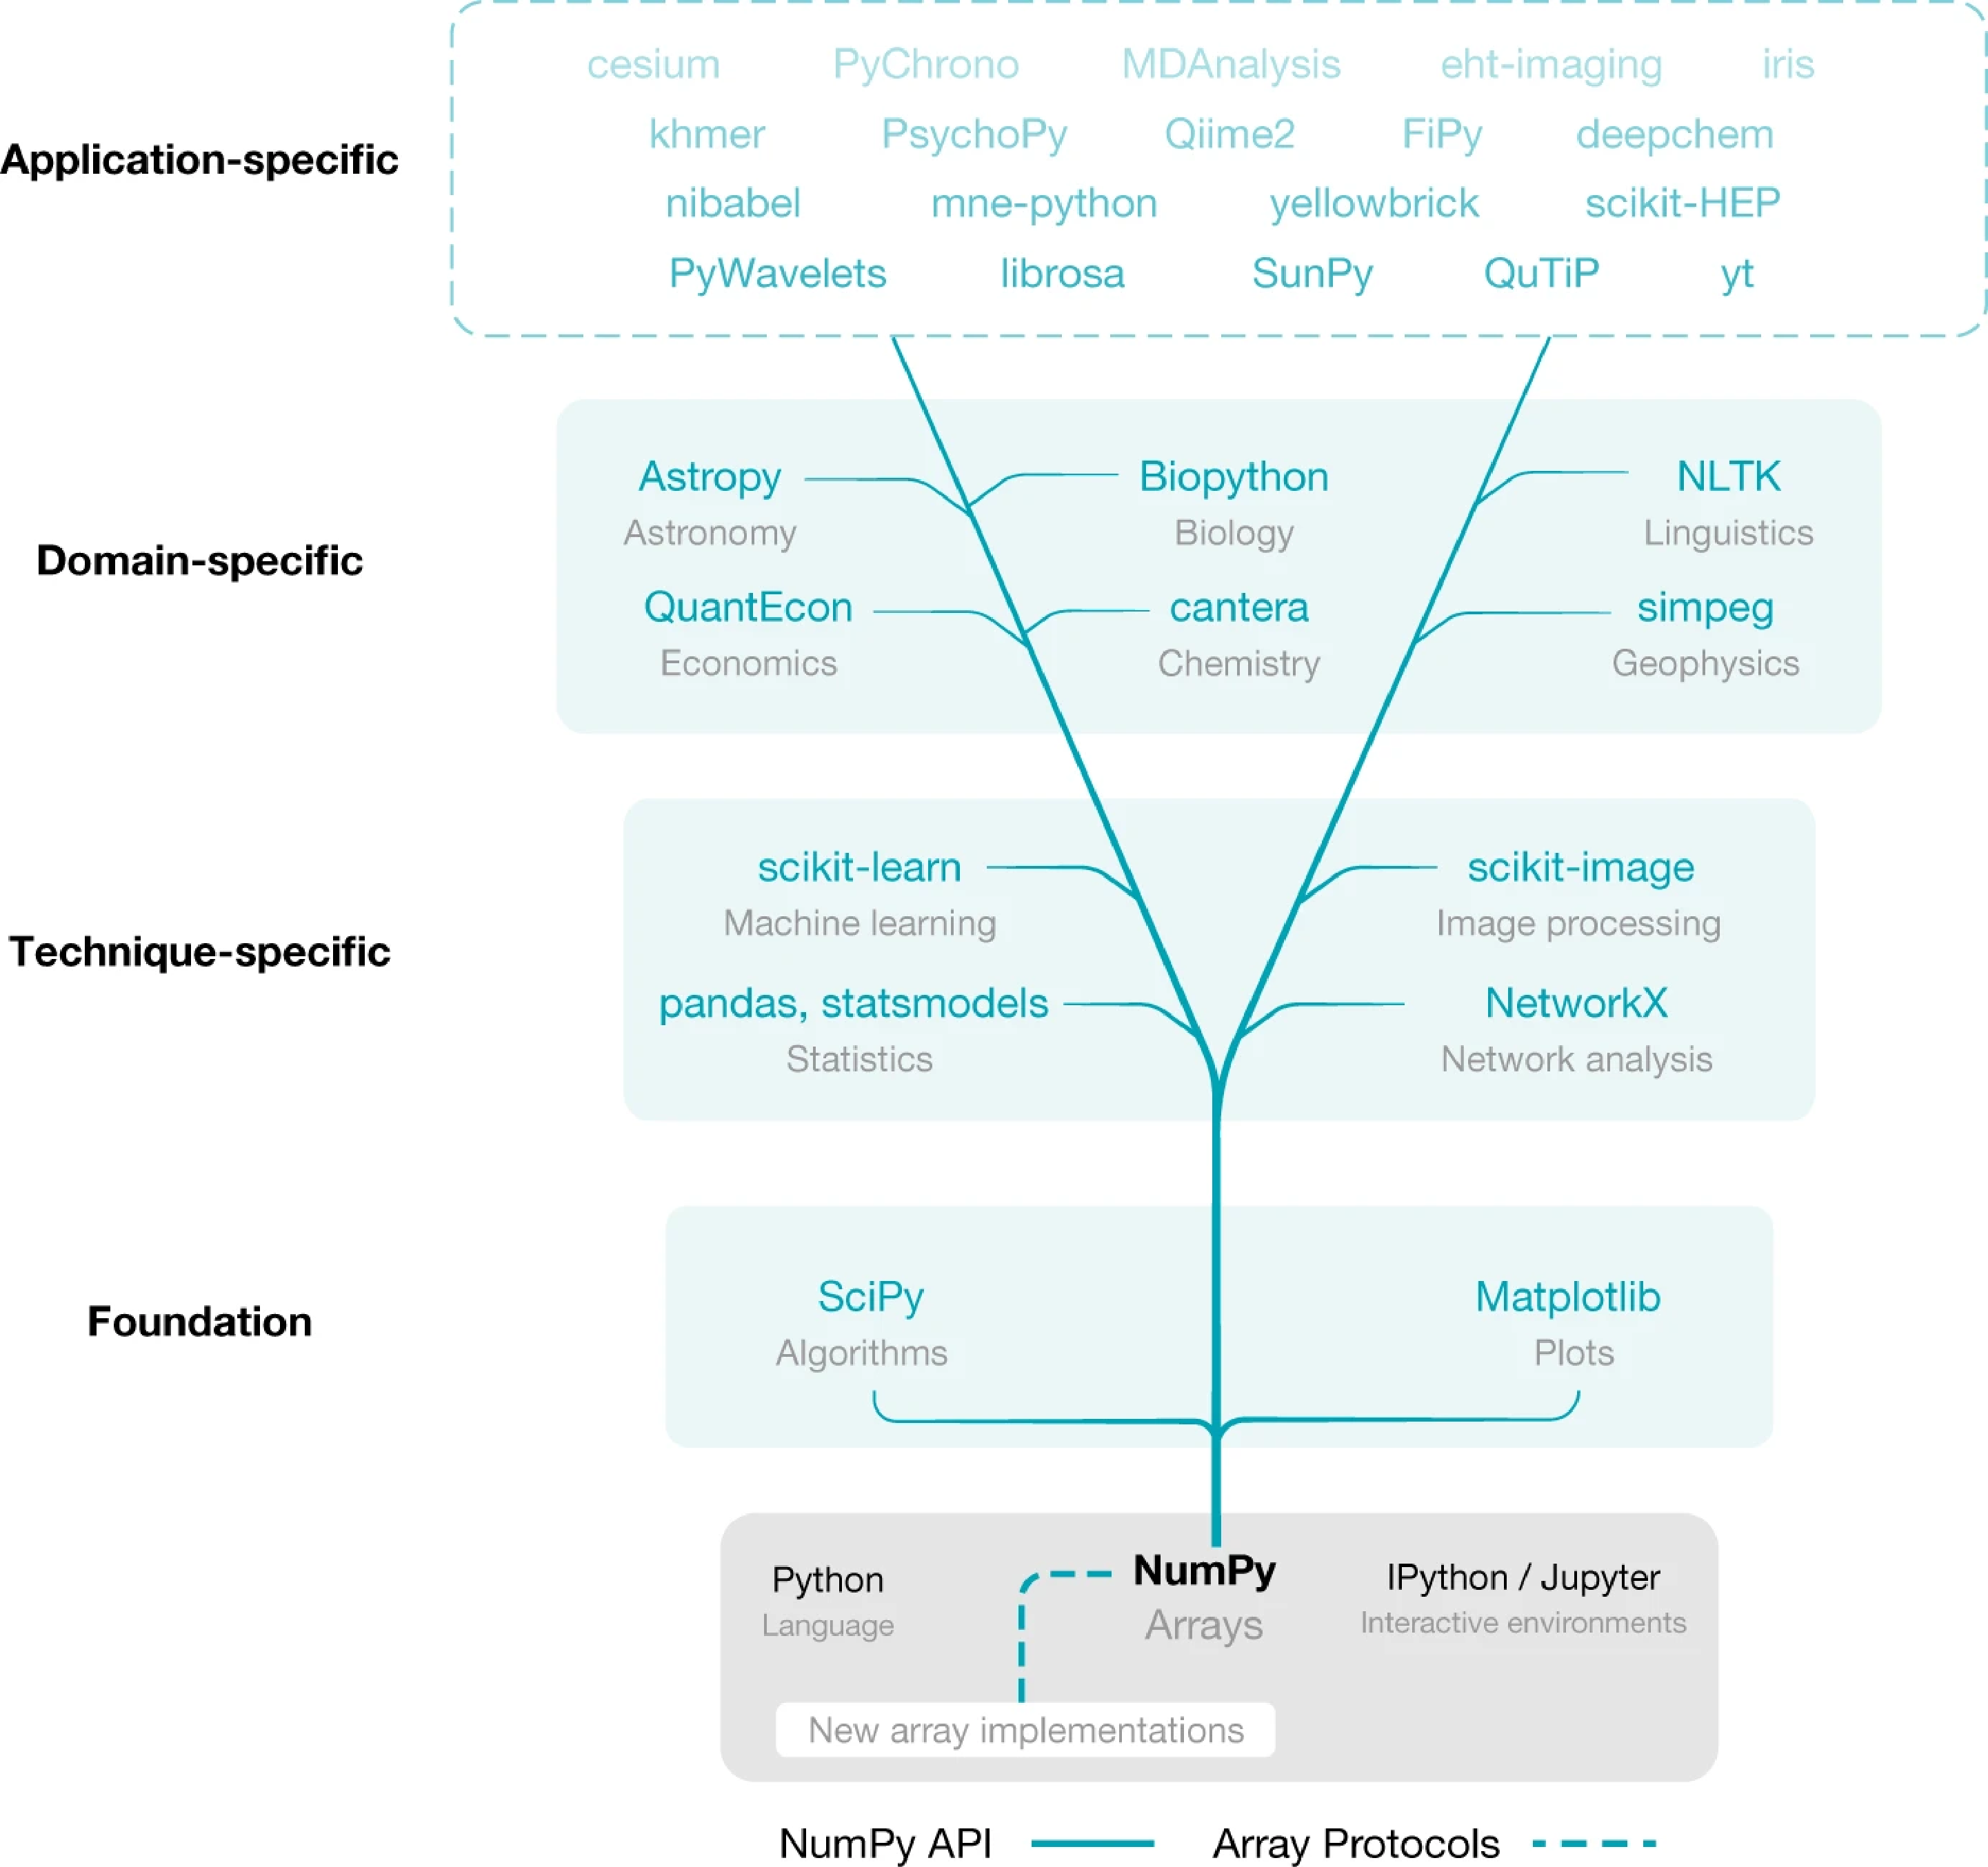
\includegraphics[width=0.8\textwidth]{./figs/numpy.pdf}
\caption[Example of hierarchical software design]{Example of hierarchical software design. Originally published with
the following caption: NumPy is the base of the scientific Python ecosystem~\cite{harris2020array}.}
\label{fig:disc_numpy}
\end{figure}

While this exercise could be conducted across arbitrary domains, if one had to make an \textit{a priori} set of
guidelines to follow it would unsurprisingly be that higher quality datasets, simpler problems, and more open and
widely tested code will generally lead to more consistently stable solutions.


\subsection{Future Directions in Operationalizing Perturbation Analysis}
The initial aim of this thesis was to identify instabilities within neuroimaging pipelines. An exciting evolution
of this plan was the finding that the variability arising from numerical perturbations may contain meaningful signal.
This suggests that perturbation analysis is not only valuable as a tool for measuring the stability of algorithms or
workflows, but that it can be applied far more flexibly to improve their quality. Considering this, next steps in
this area could be categorized into two broad questions: \textit{where} to perturb, and \textit{what} to do with the
induced variability. I will discuss different components of neuroimaging workflows which may benefit from perturbation
analysis and identify several possible applications of the results for each. I will then more broadly discuss other
applications for perturbation analysis and possible open questions as they may apply across each of these areas.

\subsubsection{Targets for Perturbation}

Neuroimaging data undergoes considerable processing after collection, beginning with image reconstruction. Initiatives
such as Gadgetron~\cite{hansen2013gadgetron} provide scanner-agnostic MRI reconstruction algorithms in an effort to
both improve the quality of these reconstructions and reduce cross-vendor variances. The perturbation of image
reconstruction algorithms could be performed to identify which algorithms are the most robust across a set of
manufacturers and scanner models. In addition to the identification of robust reconstruction methods, higher fidelity
images could be generated through the ensemble of perturbed images, possibly achieving benefits like those found in
High Dynamic Range image enhancement. Similarly, this could be applied to influence the development of vendor-neutral
pulse sequences themselves~\cite{karakuzu2020qmrlab}, and inform the adoption of stable data
collection-and-reconstruction pairs.

Reconstructed images typically undergo numerous alignments, corrections, denoising steps, and modelling prior to their
application in the modelling of structural or functional phenomena. These processing steps, such as image registration
which is relevant across all modalities of neuroimaging, are often known to exhibit sensitivity to initial conditions
or noise~\cite{salari2020file}, as was confirmed here. The perturbation of any of these components or entire workflows
could be done to test the sensitivity of specific components to numerical error or identify unstable steps within
pipelines.

Processed data are often terminally used in statistical testing or machine learning frameworks. Commonly used
frameworks for testing hypotheses or fitting models often contain an element of randomness, such as Permutation
Testing~\cite{oden1975arguments} or Stochastic Gradient Descent~\cite{bottou1991stochastic}. This tolerance and
expectation of randomness likely makes them less susceptible to the errors associated with minor perturbations.
However, feature selection, a typically deterministic process, is commonly performed on neuroimaging data prior to
their application in these frameworks~\cite{mwangi2014review}. In cases where initialization of these features has
considerable impact on their quality~\cite{kobak2021init}, the perturbation of both the initializations and feature
selection algorithm itself serves as an interesting avenue for exploration. It is possible that perturbing feature
selection will lead to similarly meaningful variability as was observed here, which would have the considerable benefit
of being much less computationally expensive than the perturbation of image processing steps.

\subsubsection{Applications of Perturbations \& Open Questions}

This thesis ultimately focused on two specific applications and interpretations of perturbation analyses: the
evaluation of pipeline stability and the aggregation of unstable derivatives. There are many possible extensions to
this work and distinct functions that MCA-based perturbations can enable from both the perspective of tool
development and analysis. One such opportunity from the perspective of tool development is the localization of
instabilities. VeriTracer~\cite{chatelain2018veritracer} provides functionality to trace the execution of
workflows and evaluate the propagation of numerical error throughout pipelines. By gradually improving or
removing sources of instability within pipelines, it would be possible to construct workflows that are more
robust to numerical error. In the case of neuroimaging, this can be used to identify which components of a
workflow are more susceptible to instabilities. In the experiments performed here, the pre-processing of data was
unperturbed leaving only few modelling steps as candidates for the introduction of instabilities. However, in
typical analytical settings where the two steps are performed sequentially by a single pipeline, the localization
of instabilities would serve as an important prerequisite for pipeline improvement. This would further allow the
manipulation of instabilities such that in settings where uncertainty is viewed as a bug it could reduced, or in
cases where added variability may be desired it these steps could be further perturbed.

A separate approach to pipeline modification would be to introduce a mixed (declining) precision model for
data in pipelines. In this case, MCA could be used to estimate the number of significant bits at each node of
a pipeline, and use this information to truncate the data and bit-space allotted to subsequent results accordingly.
This approach would not only remove the compounding effect of numerical instabilities at each node (as defined at a
context- and tool-appropriate resolution), but it would make explicit a priority for tool developers to err on
the side of building simpler and more robust pipelines. In a preliminary exploration of this idea, I truncated the
data associated with Chapter~III after pre-processing was performed and found that a large portion of the induced
variance in connectome construction was reduced in the sparse instrumentation case.

In cases where the re-engineering of pipelines is either non-feasible (e.g. closed source software) or not of
interest, Chapter~IV demonstrates that capturing the induced variability can improve the quality of derived results.
An interesting comparison can be made here between pipeline variability and the Bias-Variance trade
off~\cite{jain2000statistical}. Deterministic pipelines without perturbations will produce a single result with a
single fixed (and biased) error. When perturbations are introduced, this error shifts from a single biased quantity
to distinct errors with considerable variability. Rather than then considering any single result of the tool as the
``true'' result, we can model a series of results derived from the same data in the form of a \textit{mean} $\pm$
\textit{variance}, for example. This shift in perspective is powerful: statistics have long concerned themselves
with accounting for measurement error in the collection of samples and developing robust measure for estimating
population-level statistics. Adopting such techniques across perturbed observations will not only allow for more
richly descriptive individual measures, but it will provide a quantitative value of measurement uncertainty which
can be accounted for in subsequent testing and modelling efforts. This would enable the construction of a joint
false-positive rate when combining the uncertainty in results and testing frameworks, and would lead to more
reproducible findings.

Finally, a point which was mentioned here is the distinction between unique MCA instrumentations. The comparison
between the two instrumentations explored here provides perhaps the simplest case for such a comparison: the
sparse environment induced perturbations on a strict subset of the operations perturbed in the dense setting.
However, when considering pipelines built upon different libraries, such as the dependence of
FSL~\cite{Jenkinson2012-ly} on many Libmath functions~\cite{salari2020file} versus the dependence of
DIPY~\cite{Garyfallidis2014-ql} on Python, these instrumentations become increasingly difficult to compare. In an
extreme case where all floating point operations are instrumented with MCA for both pipelines, we can ignore this
problem and state that true MCA is applied in both cases. This claim is fragile, however, as even if a single
operation or function is unperturbed in either case, there is the possibility of either allowing for the unequal
propagation of errors, or the unfair ``skipping'' of a highly (un)stable step; this picture becomes further
muddied as instrumentations become even less dense. While this may not be a substantial issue in practice, as the
variability of results will likely be explored within a given tool and subsequent stabilities could be compared,
this problem of comparing instrumentations can arise within a pipeline, as well. For example, the instrumentation
of the DIPY-constructed pipelines that were tested throughout this thesis was performed with
Verificarlo~\cite{Denis2016-wo}. Using this tool, BLAS, LAPACK, NumPy, the Python interpreter, and Cython
libraries associated with DIPY were all re-built with MCA-logic introduced at the level of C or FORTRAN. If the
instrumentation was instead introduced from the level of Python as function decorators, for example, experiments
performed across the two versions would capture distinct and possibly non-overlapping variability. The
relationship between distinct instrumentations in general is poorly understood, and there currently doesn't exist
a theoretical framework for their comparison. Development of such an understanding, possibly with roots in Set
Theory~\cite{jech2013set}, would be an extremely interesting topic for further investigation that would increase
the generalizability of findings derived from perturbation experiments.


\subsection{Hindsight}
The final topic I would like to discuss is centred on hindsight. Throughout this project I have developed tools
for scientific infrastructure, built pipelines from modular pre-existing components, adapted a numerical analysis
framework to a new scientific domain, modelled instability in connectomes through a wide array of both commonly
used and novel measures, and showed how numerical instability can be a useful property of software\footnote{An
observation consistent with the famous justification for the bagging of predictors in machine
learning~\cite{breiman1996bagging}}. This process has not only been punctuated by scientific outputs which found
their ways into papers, but by failures and lessons, both pertaining to my own work and the field of neuroimaging
at large. I have published successes and failures from my Ph.D. on my website throughout my
degree\footnote{\url{https://gkiar.me/phd}} in an effort to not repeat my own mistakes and allow others to learn
from them. While making an effort to be brief, I feel it necessary to provide some considerations and advice that
would be relevant both to my previous-self and possibly the field of neuroimaging as a whole. None of these
reflections are intended to be perfect, but merely serve as some things to think about...

\paragraph*{Be Aware of the Cost of Computing}
While this advice may at first provoke thought about funding and the cost of either building machines or using the
cloud, I do not intend to refer to money, but energy. Scientific computing is an expensive endeavour: over the course
of my thesis, I have consumed nearly $22$ CPU-years worth of execution time for the project directly related to my
thesis, and double that if considering collaborations. Even taking a lower-bound estimate, this means my experiments
have consumed $4,000$ kWh of electricity\footnote{\url{https://www.top500.org/lists/green500/2019/11/}}. I have been
fortunate to perform my research on computers residing in Quebec and Ontario, where my average rate of Carbon
emissions at the time of writing was approximately $20$ g CO\textsubscript{2}/kWh\footnote{\url{http://bit.ly/canada-energy-consumption}}.
In this relatively green environment my research has produced $160$ kg CO\textsubscript{2} emissions which, for
reference, currently equates to an upper-bounded offset cost of approximately $\$8.00$\footnote{\url{https://www.energysage.com/other-clean-options/carbon-offsets/costs-and-benefits-carbon-offsets/}}.
If I had performed my experiments in another environment, such as through Amazon Web Services instances residing in
the United States where the rate of Carbon emissions averages over $400$ g CO\textsuperscript{2}/kWh\footnote{\url{https://www.eia.gov/tools/faqs/faq.php?id=74}},
the total environmental footprint would increase $20$-fold, which would amount to the same Carbon footprint as putting
and extra car on the road for a year\footnote{\url{https://www.nrcan.gc.ca/sites/www.nrcan.gc.ca/files/oee/pdf/transportation/fuel-efficient-technologies/autosmart_factsheet_6_e.pdf}}!
This is not meant as an endorsement for running analyses in Canada \textit{per se}, but merely as a reminder that we
should be aware of the impact that our experiments have on the world more broadly than just our papers. This is
important so we can clearly evaluate which experiments are worth doing and offset any distant harm we may cause.

\paragraph*{Keep Clear and Incremental Objectives}
Over the last several years it has become clear to me that projects are rarely ``complete''. There is always
another experiment, figure, analysis, or interpretation that we can explore. However, the longer we follow these
rabbit holes (which often provide their fair share of excitement), I have found it becomes gradually easier to lose
sight of the original target or purpose. The experiments I presented in Chapter~IV, for example, are a small
subset of the models, conditions, and experimental permutations originally considered when aggregating connectomes.
I did not exclude the others because of their outcomes, but because they failed to answer the question I sought out
to explore. These incrementally distinct experiments were the result of asking new questions that brought me not
only further from where I started, but into the territory of having answers that were ultimately uninterpretable
because I hadn't fully answered questions that they depended upon. I got momentarily swept up in where I wanted my
project to lead eventually, rather than taking the time to fully understand where it was now. I suspect that I am
not the only scientist to fall into this trap, and I believe the field of neuroimaging as a whole may have
experience with it, at least in appearance. Despite regularly defining possible real-world applications and outcomes
in papers, neuroimaging and fMRI in particular has received considerable criticism for lack of delivering on this
promise~\cite{robinson2004fmri}. While this criticism is perhaps unfairly harsh~\cite{lyon2017dead}, it remains that
neuroimaging hasn't yet become as relevant as may have once been anticipated. While I believe this is in part due to
an academic curiosity taking the reins as I experienced, I think this in reality is more of an ``image problem'' due
to conflation of the \textit{eventual} objectives and those which are presently feasible and being built towards. I
do not mean to discourage exploration or the ``accidental findings'' that are so necessary to science, but merely
that the evaluation of progress towards clear objectives should be emphasized, so that both as scientists and the
public we can disentangle the two and more effectively steer our work towards initiatives that are both academically
and practically relevant. By clearly defining and communicating our goals and the incremental objectives that must be
met along the way, both as individual scientists and as a field, I suspect we'll stop having to defend the reality
that science is an incremental and non-linear process that takes time. 

\paragraph*{Avoid ``Not Invented Here'' Thinking}
A point which I have mentioned repeatedly throughout this thesis is that there are a considerable number of
libraries that have been built to accomplish similar tasks, often in isolation. In fact, I committed this taboo
myself during this thesis in Chapter~I with the creation of Clowdr. I built this tool out of the necessity to run
experiments in the particular way I had envisioned, and I did so largely making use of existing components but
separate from any similarly-aimed efforts. As a result, the code has at various points required development to
function in new use cases or become difficult to maintain as its sole core contributor. In retrospect, a more
sustainable solution may have been for me to build my extension into an existing framework or library, such as
Nipype~\cite{gorgolewski2011nipype} or CBRAIN~\cite{sherif2014cbrain}. While the creation of this tool was
necessary and relevant for the completion of my thesis, if I built the extensions I needed in an existing ecosystem
I would have not only gained the review and debugging support of its user and developer base, but also been able to
provide a more accessible contribution to the community who were already familiar with a given environment. As my
thesis progressed, I learned from this and contributed more clearly, through Fuzzy, back to the Verificarlo
ecosystem. I believe the same inefficiency I presented with my development process of Clowdr could likely be said for
many tools that have been built in neuroimaging (and likely science more broadly), and perhaps even exacerbated based
on the level of adoption of existing lower-level tools. Though I don't believe there should be a single solution for
every challenge, I do think that maintaining a collaborate-first and compete-second perspective would not only reduce
possible redundancies in a given space, but would lead to higher quality and more sustainable contributions.

